\documentclass[conference]{IEEEtran}
\IEEEoverridecommandlockouts
\usepackage[utf8]{inputenc}

\usepackage{url}
\usepackage{cite}
\usepackage{caption}
\usepackage{amsmath,amssymb,amsfonts}
\usepackage{algorithmic}
\usepackage{graphicx}
\usepackage{textcomp}
\graphicspath{{figures/}}
\usepackage{xcolor}
\usepackage{float}
\usepackage{caption}
\captionsetup[figure]{skip=0pt}
\usepackage{hyperref}
\usepackage{float}
\usepackage{booktabs}
\usepackage{xurl}
\def\BibTeX{{\rm B\kern-.05em{\sc i\kern-.025em b}\kern-.08em
    T\kern-.1667em\lower.7ex\hbox{E}\kern-.125emX}}
\begin{document}

\title{Data-Driven Modeling of Particle Transport and Tracking Evolution in Complex Media\\
{\footnotesize \textsuperscript{}
}}

\author{
\IEEEauthorblockN{Melanie Melkonyan}
\IEEEauthorblockA{Zaven P. and Sonia Akian College\\
of Science and Engineering\\
American University of Armenia\\
melani\_melkonyan@edu.aua.am}
\and
\IEEEauthorblockN{Aleksandr Hayrapetyan}
\IEEEauthorblockA{Zaven P. and Sonia Akian College\\
of Science and Engineering\\
American University of Armenia\\
ahayrapetyan@aua.am}
}


\maketitle

\begin{abstract}
Understanding particle transport in complex anisotropic media is an important problem in soft matter physics, particularly in liquid-crystal systems where particle motion is influenced by orientational order, defect structures, and external fields. These conditions create complex optical backgrounds and dynamic particle behavior, making reliable detection and long-term trajectory reconstruction difficult. This work proposes a data-driven pipeline for particle detection and tracking in free-surface liquid crystal (FSLC) microscopy videos. Particles are first detected per-frame using a fine-tuned YOLO object detector, and then, a small set of high-confidence detections initializes tracking for each expected particle. Each initialization is propagated into a continuous trajectory using SAM 2 - a video segmentation model that maintains identity-preserving object masks across frames. Then, motion-based post-processing stage merges fragments with consistent spatial and velocity behavior to recover stable particle identities. Evaluated on videos containing one to three particles, the method produced stable trajectories in single-particle and well-separated multi-particle cases, establishing a viable approach for data-driven particle detection, tracking, and trajectory reconstruction in complex liquid-crystal environments. 
\end{abstract}

\begin{IEEEkeywords}
Deep learning, free-surface liquid crystal, multi-object tracking, object detection, particle trajectory reconstruction, Segment Anything Model 2, YOLO
\end{IEEEkeywords}


\section{Introduction}
Particle transport in complex anisotropic media is a fundamental problem in soft-matter physics. In free-surface liquid crystal (FSLC) films, a focused laser drives microparticles into oscillation, rotation, and combined motion patterns \cite{shvetsov2024}. Reliably detecting each particle in every frame and maintaining its identity across thousands of frames is the central computational challenge addressed in this work.

The motion modes observed in FSLC systems are the experimental signature of the underlying physics, and their quantitative analysis (period, amplitude, phase, radius) depends on accurate trajectories. Manual or visual tracking does not scale to the long recordings needed to resolve these dynamics, and the imaging conditions - cluttered optical backgrounds, deformable particle appearance, deterministic non-Brownian motion, frequent close encounters - make automated tracking non-trivial.

Classical particle trackers such as TrackPy \cite{allan2021_trackpy} were developed for systems with approximately Gaussian intensity profiles and near-Brownian motion, which differ from the conditions encountered in FSLC microscopy. General-purpose multi-object trackers such as BoT-SORT \cite{aharon2022_botsort} and ByteTrack \cite{sheng2023_yolov7_bytetrack} were designed for rigid objects in natural-scene video and do not transfer cleanly to anisotropic microscopy. Deep-learning models such as YOLO (You Only Look Once) \cite{vijayakumar2024_yolo_review} for detection and SAM 2 (Segment Anything Model 2) \cite{ravi2025_sam2} for promptable video segmentation have shown strong performance on standard benchmarks, but their application to FSLC microscopy has not yet been explored. 

To address these gaps, this work develops and evaluates a three-part data-driven pipeline for particle detection, tracking and trajectory reconstruction in free-surface liquid crystal (FSLC) microscopy videos. 


\section{Literature Review}
Particle dynamics in liquid crystal (LC) systems have been studied as a platform for soft-matter manipulation, with electric fields, thermal gradients, and optical excitation used to drive controlled particle motion \cite{lavrentovich2014_transport_particles_lc}. In free-surface LC films, focused-laser irradiation produces Marangoni convection coupled to elastic deformations of the director field that drives microparticles into oscillation, rotation, and combined oscillatory–rotational trajectories \cite{shvetsov2024}. The quantitative analysis of these trajectories provides the experimental signature of the underlying flow and elastic structure, which makes reliable particle detection and tracking very important.

Liquid crystals are particularly challenging environments for automated particle analysis because they combine fluid motion with long-range orientational order and strong sensitivity to external stimuli such as temperature, electric fields, and optical excitation. As a result, microscopy images of LC systems often contain non-uniform illumination, evolving optical textures and topological defects that change dynamically over time. Recent reviews on machine learning in LC research show that these characteristics create very complex visual environments that are difficult for traditional computer-vision approaches to analyze reliably \cite{khan2025_ml_liquidcrystals}. In addition, LC systems frequently display nonlinear phase behavior, overlapping textures, and anisotropic transport, which makes segmentation, localization, and trajectory reconstruction much more difficult than in conventional isotropic fluids \cite{khan2025_ml_liquidcrystals}.

The Crocker–Grier algorithm \cite{crocker1996_digital_video_microscopy} and its Python implementation TrackPy \cite{allan2021_trackpy} remain the standard tools for particle tracking in microscopy. The method achieves sub-pixel localization on well-separated bright spots and is widely used in colloidal microrheology and single-molecule studies. Its main weakness is sensitivity to background texture, illumination changes, and motion that deviates from near-Brownian dynamics, making it unsuitable for FSLC microscopy conditions. 

Classical digital video microscopy methods also rely heavily on manually selected thresholds and user-defined assumptions about particle appearance. These assumptions typically include homogeneous illumination, approximately spherical particle shapes, and stable imaging conditions. Under low signal-to-noise ratios or dynamically changing backgrounds, their performance becomes even worse \cite{helgadottir2019digitalvideomicroscopy}. Helgadottir et al. introduced DeepTrack, a convolutional neural-network-based alternative to traditional particle localization methods. Their work demonstrated that deep-learning approaches can achieve robust sub-pixel localization even under noisy or non-uniform illumination conditions where classical algorithms fail \cite{helgadottir2019digitalvideomicroscopy}. This work established an important transition in microscopy analysis: instead of relying on manually written rules, learned models can automatically extract visual features directly from data. However, DeepTrack mainly addresses particle localization in individual frames and does not solve the long-term identity-preservation problem required for trajectory reconstruction.

Learned object detectors replace classical algorithms with features learned from data. The YOLO family \cite{vijayakumar2024_yolo_review} predicts bounding boxes in a single forward pass and has been applied to cell counting, particle identification, and defect detection in LC textures. It is robust to appearance variation and complex backgrounds. Its limitation, however, is that detection is performed independently on each frame: YOLO has no temporal memory and produces no identity correspondence between frames. By itself, it solves the localization problem but leaves the trajectory problem open.

Recent studies in particle tracking increasingly combine deep learning with multi-object analysis to address crowded and noisy environments. Xu et al. proposed a deep-learning-based multiple-particle tracking framework using multilayer perceptrons and multi-output models for tracking particles in complex systems \cite{xu2024_dl_multiple_particle_tracking}. Their work emphasized that conventional methods often fail in the presence of particle overlap, irregular illumination, and noisy backgrounds \cite{xu2024_dl_multiple_particle_tracking}. The proposed framework demonstrated that learned representations can improve robustness in difficult imaging conditions and allow simultaneous tracking of multiple particles. Nevertheless, the method still depends on framewise prediction and does not explicitly address identity preservation during long interactions or close particle encounters, which are main difficulties in FSLC systems where trajectories can overlap frequently.

Identity-preserving tracking is conventionally addressed by tracking-by-detection methods, which pair a learned detector with a frame-to-frame linker. BoT-SORT \cite{aharon2022_botsort}, ByteTrack \cite{sheng2023_yolov7_bytetrack} methods perform well on natural-scene benchmarks such as MOT17 and MOT20, where objects are rigid and visually consistent. Their underlying association logic, however, is built around bounding-box overlap and short-term motion priors learned from natural video, both of which become unreliable when objects are deformable, partially merge during close encounters, or move with strongly non-translational dynamics.

In dense particle systems, where trajectory reconstruction becomes difficult, nearby particles frequently overlap visually or move collectively. Recent work by Zhang et al. introduced a video flow-informed neural network (VFINN) for high-density particle tracking using dense optical-flow learning \cite{zhang2025largevisionmodeltracking}. Their method estimates pixel-level flow fields directly from sequential microscopy images and uses these flow estimates to guide temporal linking between particles. By learning a global motion field instead of relying only on local frame-to-frame matching, VFINN improved tracking robustness in biologically complex systems. However, the approach was primarily designed for dense diffusion-dominated systems and optical-flow estimation. It does not explicitly address identity preservation in oscillatory particle dynamics with repeated trajectory crossings, which are characteristic of our FSLC experiments.

Another recent direction combines deep learning with physical modeling. Physics-informed learning approaches attempt to integrate known physical constraints directly into neural-network architectures instead of treating trajectories purely as abstract data. Zhang et al. proposed the stochastic particle-informed neural network (SPINN), which incorporates stochastic differential equations into deep-learning-based trajectory analysis \cite{zhang2025physicsinformedstochasticparticle}. Their framework separates deterministic and stochastic components of motion while analyzing diffusion behavior at single-frame temporal resolution. The motivation behind this work is that conventional statistical approaches often require large datasets and stationary assumptions that do not hold in heterogeneous or rapidly evolving systems \cite{zhang2025physicsinformedstochasticparticle}. Physics-informed methods improve interpretability and help reveal hidden transport mechanisms, but they generally focus on diffusion characterization after trajectories are already obtained. In other words, they improve trajectory analysis rather than solving the initial multi-object tracking and identity-preservation problem itself.

A more recent direction is promptable foundation models for video segmentation. SAM 2 \cite{ravi2025_sam2} propagates a prompted object's identity across frames through an internal memory mechanism, providing identity preservation across long sequences from a single prompt. Its limitation is that it does not decide what to track, and this requires an external mechanism to select prompts and manage multi-object identity.

Each of these three categories - classical trackers, learned detectors with tracking-by-detection, and promptable video segmentation - addresses one part of the trajectory-reconstruction problem well but leaves the others open. Our work integrates these three directions into a single end-to-end pipeline for particle detection and tracking in anisotropic microscopy.

\section{Methodology}

\subsection{Dataset and Experimental Source}
The dataset was provided by the Institute of Physics and contains 13 experimental microscopy videos, recorded following the experimental configuration of Shvetsov et al. \cite{shvetsov2024}. The recordings capture 3 $\mu m$ silica particles in free-surface liquid crystal (FSLC) films under localized optical excitation, where a focused laser beam locally heats the substrate beneath the LC film and induces Marangoni convection coupled to elastic deformations of the director field \cite{shvetsov2024}. Microparticles trapped near the beam axis exhibit motion modes such as oscillation, rotation, and combined oscillatory-rotational ("nutation-like") trajectories. The resulting anisotropic optical backgrounds, complex particle trajectories, and frequent close interactions make robust detection and long-term identity tracking very challenging.

\begin{figure*}[t]
\centering
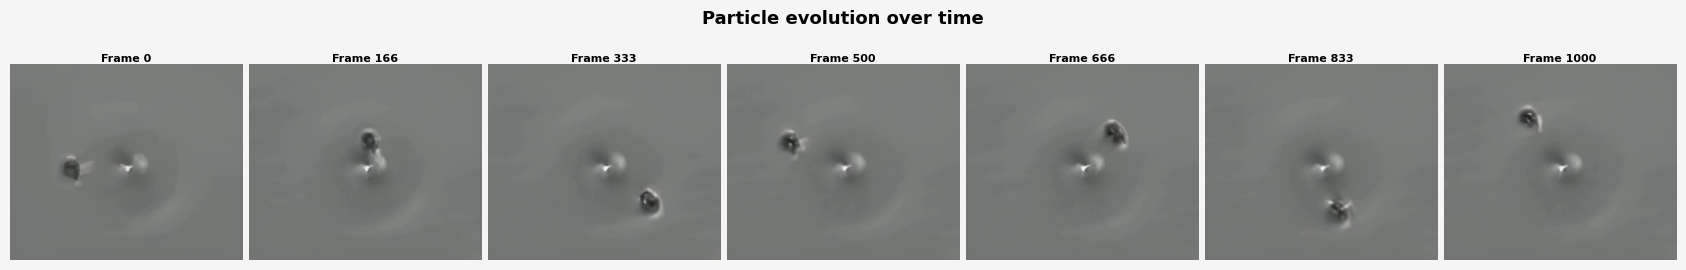
\includegraphics[
  width=0.95\textwidth,
  keepaspectratio
]{particle_evolution_over_time.png}
\caption{Particle evolution over time in one of the FSLC recordings, sampled at uniformly spaced frames.}
\label{fig:particle_evolution}
\end{figure*}

To be able to systematically evaluate the proposed pipeline along a single controlled axis, three videos were selected that isolate the effect of particle count - one-, two-, and three-particle configurations - while keeping the experimental conditions comparable as well. Because the original recordings include moments in which the laser is repositioned or the optical pattern was briefly disturbed, only temporally stable parts of the video (those with a settled beam and clearly developed particle dynamics) were manually retained for analysis. Figure~\ref{fig:particle_evolution} shows a representative example of such a segment. Each such part was then spatially cropped to the central region around the laser-beam axis, and upsampled using Real-ESRGAN \cite{wang2021_realesrgan} super-resolution to improve the visibility of small particle structures. No further preprocessing was applied during inference. Properties of the final videos are summarized in Table 1.


\begin{table}[H]
\caption{Properties of the input videos used in this work.}
\label{tab:videos}
\centering
\begin{tabular}{lccccc}
\toprule
Video & Particles & Duration & FPS & Frames \\
\midrule
\texttt{one\_particle}     & 1 & 1:16 & 33 & 2516 \\
\texttt{two\_particles}    & 2 & 1:23 & 33 & 2764 \\
\texttt{three\_particles}  & 3 & 0:38 & 30 & 1139 \\
\bottomrule
\end{tabular}
\end{table}

\subsection{Problem Statement}

The task is to reconstruct per-particle trajectories from FSLC video - a per-frame sequence of coordinates with a stable identity for each visible particle. Two properties make this challenging: particle appearance changes during motion, and the background contains optical structures that locally resemble particles. Motion is also non-Brownian, with frequent close encounters. These conditions violate the assumptions of existing trackers, that motivates two simpler baselines before the final architecture.

\textbf{Classical computer-vision baseline.} A handcrafted pipeline was implemented as an interpretable baseline. Particles were detected using two-stage Gaussian background subtraction, percentile thresholding (top 0.3\%), and morphological cleanup. Detected blobs were then linked using Kalman-filter motion prediction \cite{li2010_kalman_mot}, Hungarian assignment \cite{luetteke2012_hungarian_tracking}, and appearance-aware matching costs based on region descriptors. Figure~\ref{fig:cv_baseline_1}, Figure~\ref{fig:cv_baseline_2}, Figure~\ref{fig:cv_baseline_3} illustrate the per-frame detection steps on a single-particle, two-particle, and three-particle cases, respectively. 


\begin{figure}[H]
\centering
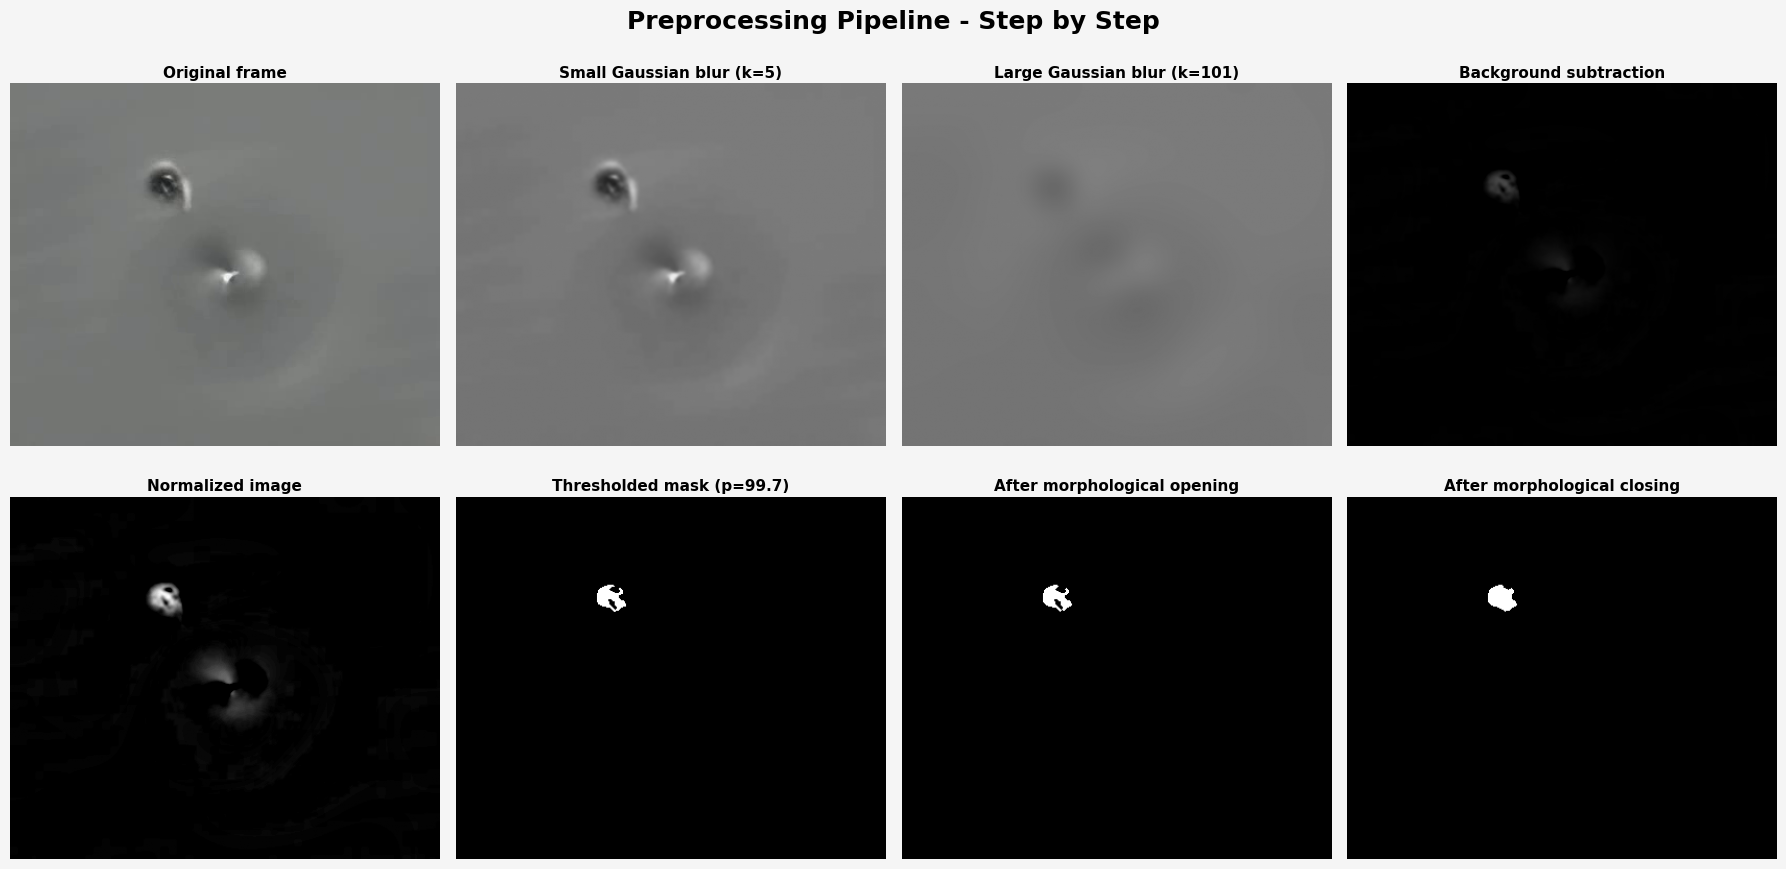
\includegraphics[
  width=\columnwidth,
  keepaspectratio
]{one particle ip.png}
\caption{One-particle Case}
\label{fig:cv_baseline_1}
\end{figure}


\begin{figure}[H]
\centering
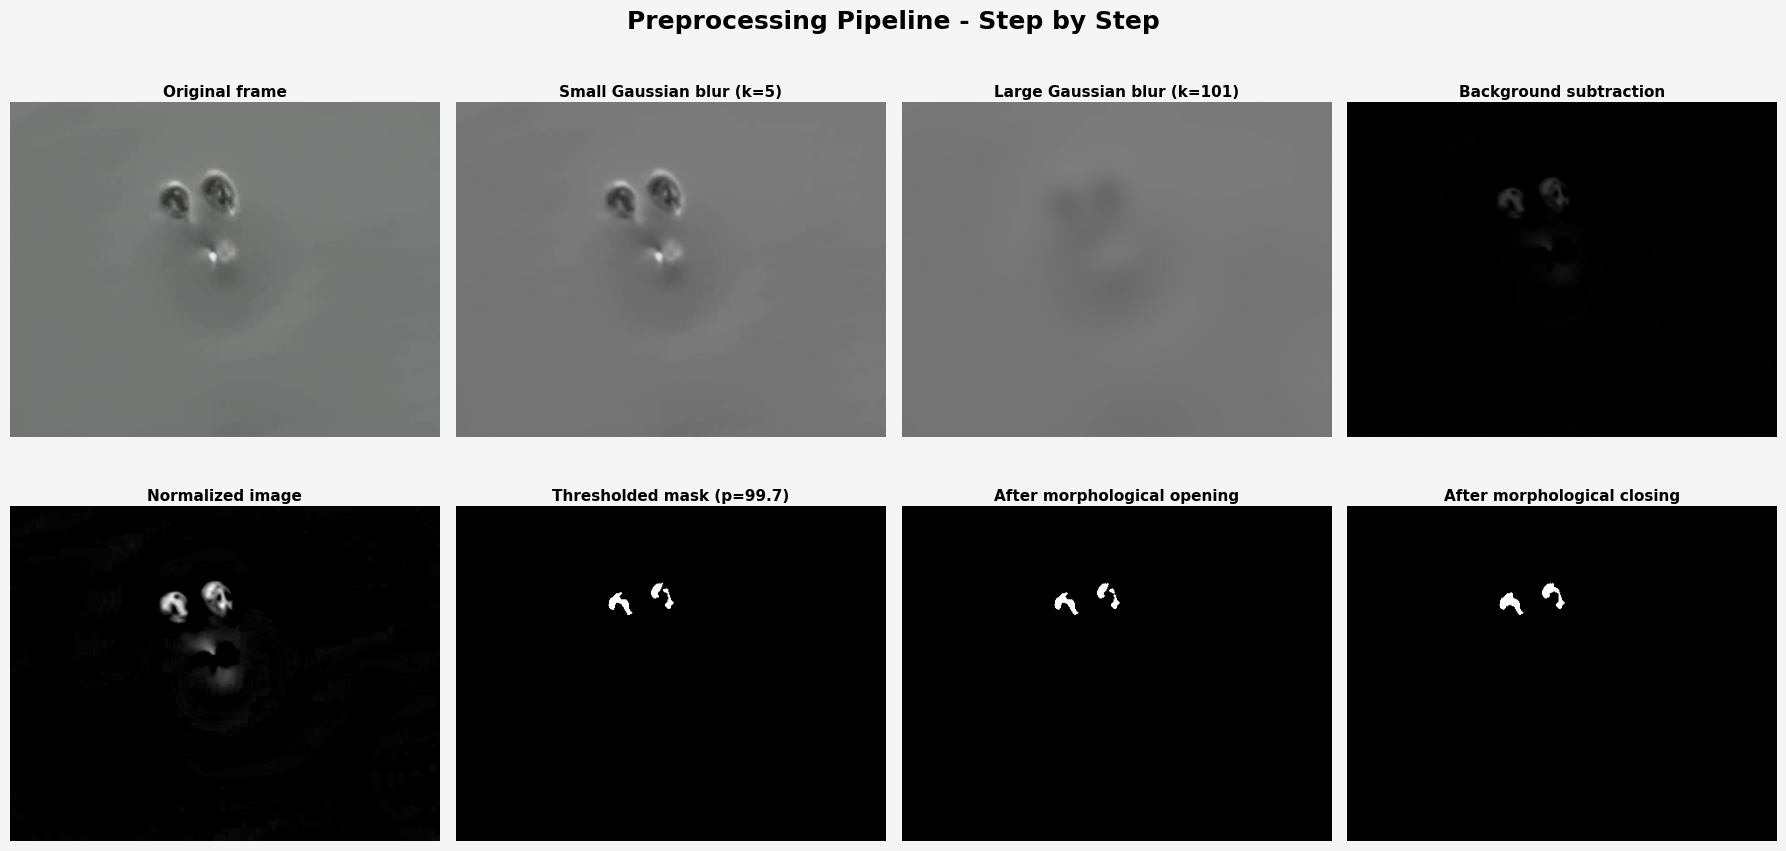
\includegraphics[
  width=\columnwidth,
  keepaspectratio
]{two particle ip.png}
\caption{Two-Particle Case}
\label{fig:cv_baseline_2}
\end{figure}


\begin{figure}[H]
\centering
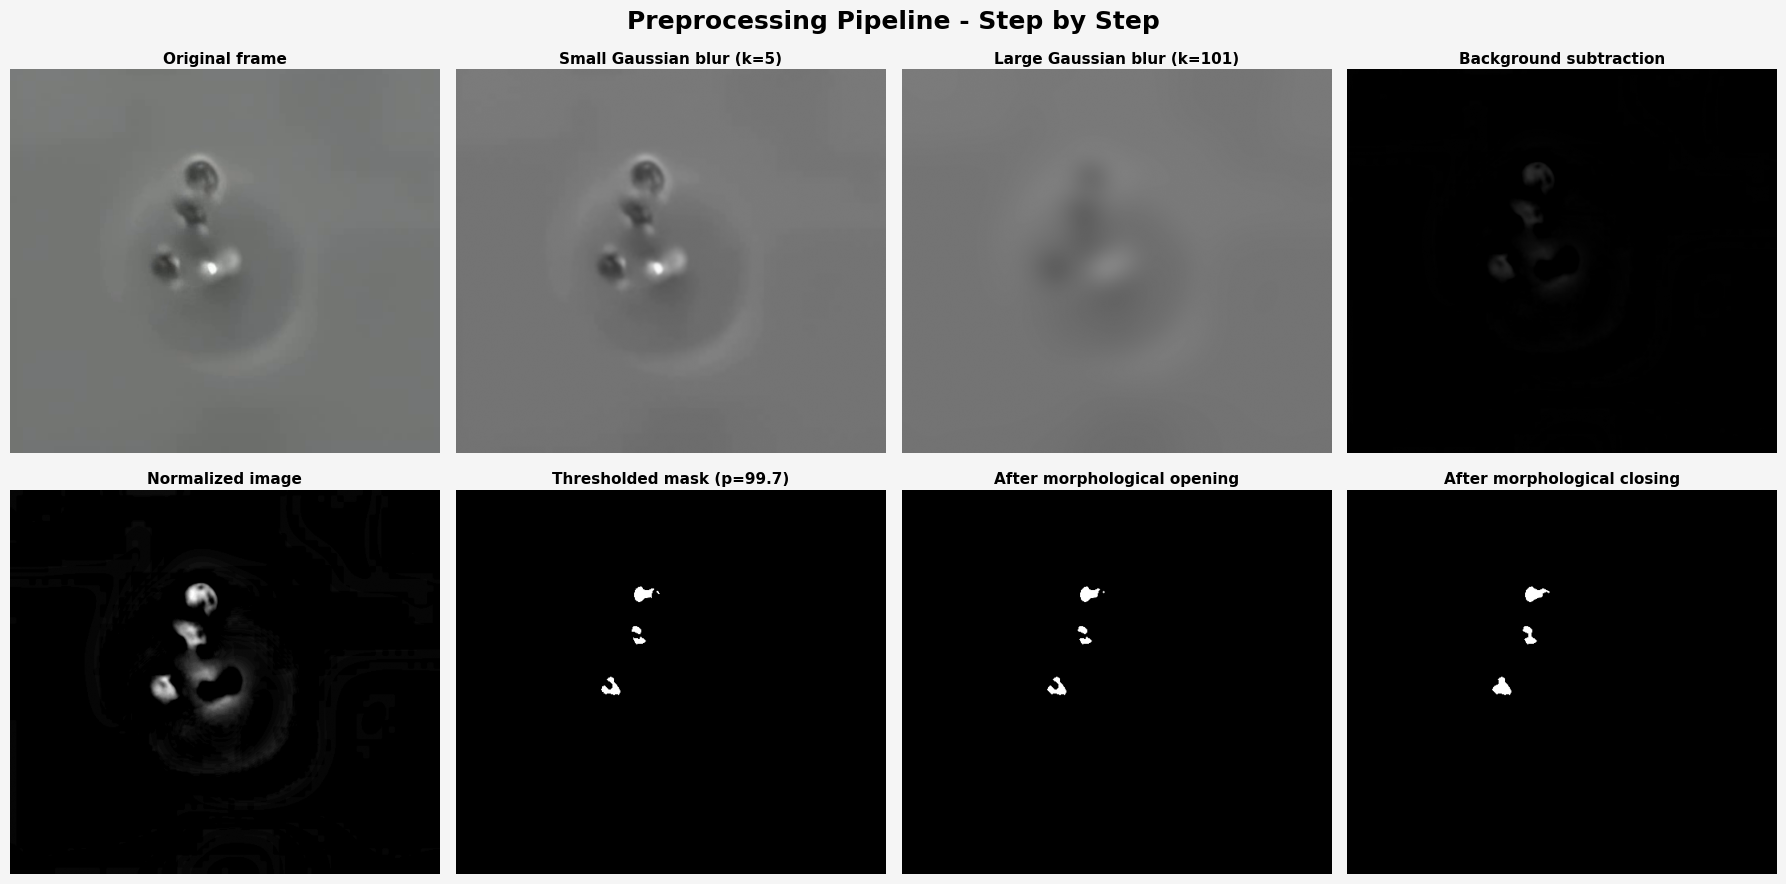
\includegraphics[
  width=\columnwidth,
  keepaspectratio
]{three particle ip.png}
\caption{Per-frame detection steps of the classical CV baseline on a three-particle frame: two-stage Gaussian blur, background subtraction, normalization, percentile thresholding, and morphological cleanup.}
\label{fig:cv_baseline_3}
\end{figure}

The pipeline failed to maintain stable identities: illumination variation, anisotropic backgrounds, and close particle interactions caused frequent identity switches, with many distinct IDs generated for a single physical particle. Initial detection was acceptable, but identity preservation was unstable even after extensive tuning of the appearance descriptors.

\textbf{Learned detector alone.} A fine-tuned YOLO \cite{vijayakumar2024_yolo_review} detector substantially improved per-frame localization, performing robustly under low contrast and complex optical textures. However, detection alone does not solve identity preservation: the model produces no temporal correspondence between frames, and missed detections, brief occlusions, or particle interactions caused identity switches and fragmented trajectories. Detection quality improved relative to the classical baseline, but long-term trajectory stability remained unreliable.

These observations motivated a hybrid architecture that combines learned detection, mask-based propagation, and trajectory-aware identity recovery, described in the following subsections.

\subsection{Microparticle Tracking Architecture}

The pipeline performs particle detection and tracking, producing stable per-particle trajectories from an input video. It consists of three parts, illustrated in Fig.~\ref{fig:pipeline}: detection and tracking stage producing trajectory fragments; a diagnostic stage for fragment inspection; and an identity-recovery stage resolving the fragments into final trajectories.

\begin{figure*}[t]
\centering
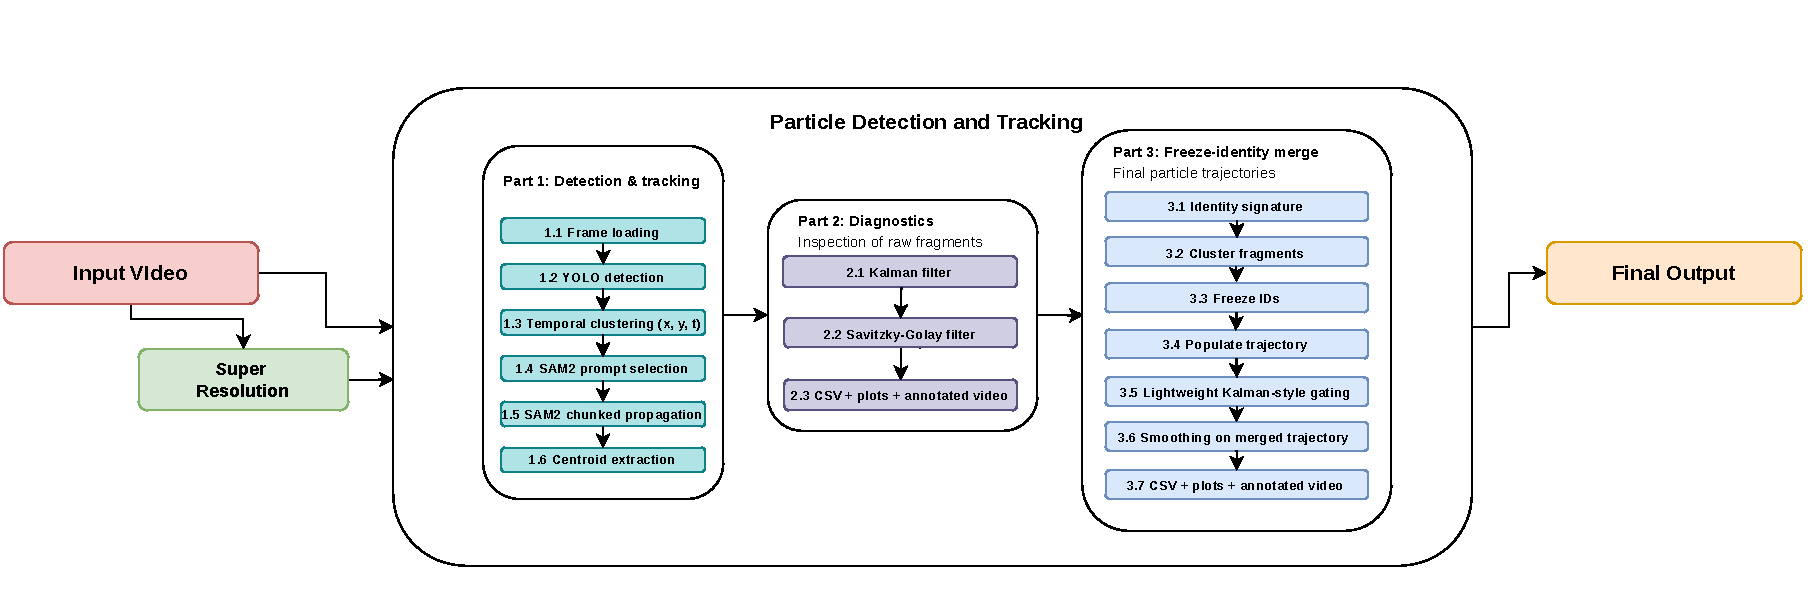
\includegraphics[
  width=0.97\textwidth,
  keepaspectratio,
  trim=0.05cm 0.5cm 0.1cm 0.5cm,
  clip
]{final final schema.pdf}
\caption{Microparticle Tracking Architecture}
\label{fig:pipeline}
\end{figure*}


\subsubsection{\textbf{YOLO Detector Training}}
A single-class YOLO detector was trained using the Ultralytics framework, starting from the pretrained YOLO26m checkpoint. Training used 360 manually annotated frames drawn from the source videos, split 288/72 between training and validation, with batch size 8, input image size 1024$\times$1024, and 80 epochs of fine-tuning under default Ultralytics augmentations. At inference, the detector produces a set of bounding boxes per frame with confidence scores; detections below confidence 0.15 are discarded, balancing recall on weakly-contrasted particles against false-positive control on background optical artifacts. The detector operates independently on each frame and has no temporal memory.

\subsubsection{\textbf{Part 1: Detection and Tracking}}
Each input video is decoded into individual frames and processed by the trained YOLO detector, producing per-frame bounding boxes. The detections from all frames are then grouped through a three-strategy cascade in fixed order, each leveraging temporal continuity differently - tracklet-based selection (linking detections across consecutive frames), stable-window selection (finding a time window of consistent detection counts), and Gaussian Mixture Model (GMM) clustering in spatio-temporal space (x, y, t) \cite{wan2019_gmm_classification} as a fallback; each resulting cluster is taken to represent a candidate particle trajectory. For each cluster, one high-confidence detection is selected as a prompt for SAM 2. SAM 2 propagates each prompt across the video in overlapping temporal chunks (3000 frames, 100-frame overlap), and the resulting segmentation masks are reduced to centroid coordinates, yielding one trajectory fragment per prompt.

\subsubsection{\textbf{Part 2: Diagnostic Fragments}}
The raw fragments produced by SAM 2 may contain small frame-to-frame jitter from mask-boundary fluctuations and brief deviations during close particle interactions. Before any identity resolution is performed, each fragment is therefore lightly smoothed in two stages. A constant-velocity Kalman filter is applied first, propagating a 2D state vector $(x, y, v_x, v_y)$ across frames; the predict step is scaled by the inter-frame gap to handle missed observations, and the update step refines the state using the SAM 2 centroid as the measurement. A Savitzky–Golay filter \cite{liu2016applications} is then applied to the smoothed positions, fitting a local low-order polynomial within a moving window to suppress residual high-frequency jitter without distorting the periodic structure of the trajectories.
The output of this stage is, for each fragment, a smoothed sequence of per-frame coordinates together with diagnostic plots and an annotated video for visual inspection. Because identity merging has not yet been performed, a single physical particle may still appear as multiple fragments at this stage; this is expected, and is resolved in Part 3.


\subsubsection{\textbf{Part 3: Freeze-Identity Merging}}
The fragments are resolved into final per-particle identities through a signature-based merging procedure. Each fragment is first summarized by a compact starting signature - its average position and average velocity computed over its first 50 frames. The starting window is intentionally chosen to capture each fragment's identity before drift between particles can accumulate during close encounters.

After that, fragments are grouped into final particle identities based on their motion signatures. Two fragments are treated as belonging to the same physical particle if their starting positions are close to each other and their initial velocity vectors are similar. These relationships are combined using a union-find structure, which merges all connected fragments into a single particle group. Each group is then assigned one final particle ID that remains fixed throughout the rest of the tracking process.

Next, the final trajectory of each particle is reconstructed frame by frame using the fragments assigned to that particle. For every new frame, a detected position is accepted only if it is close to the position predicted from the previous motion of the particle; otherwise it is rejected. If no valid position is found for more than 60 consecutive frames, the trajectory is considered finished. This step helps remove incorrect detections and prevents identity switches when particles come close to each other or cross paths.

Finally, the merged trajectories are smoothed again using the same Kalman and Savitzky–Golay filters from Part 2, but now applied to the complete unified trajectories rather than to separate fragments. The result is a stable per-frame particle trajectory with consistent identity labels.

\subsection{Evaluation Strategy}

Standard multi-object tracking metrics such as IDF1 and MOTA require per-frame ground-truth annotations, which physics-laboratory recordings of this kind do not include. Validation is therefore performed through sparse manual annotation: every 100-200th frame of each video was independently re-annotated by hand, with a bounding box drawn around each visible particle and its center treated as a manually-determined centroid. Each particle that is manually annotated is assigned a consistent identity throughout the recording. Then, the same identity is assigned to the corresponding pipeline particle in that frame, and this manual–pipeline correspondence is kept unchanged for the rest of the video. The Euclidean error between manual and pipeline centroids is computed per identity, making the metric sensitive to both localization error and identity exchange, because a swapped pair of identities would produce large per-frame distances. The same protocol is applied across all the videos.

For visualization, the matched pairs are plotted in displacement-from-start coordinates: each pipeline particle's trajectory is shown as a continuous curve representing $\|(x(t), y(t)) - (x_0, y_0)\|$, and each manual annotation is plotted as a single point at the same temporal location. This representation makes per-frame agreement directly visible and reveals identity preservation through trajectory crossings.

\subsection{Implementation and Computational Details}

The full system was organized as a three-stage pipeline consisting of detection and mask-based tracking, diagnostic fragment analysis, and identity recovery with trajectory merging. All experiments were performed on the NVIDIA A100 SXM4 GPU with 80 GB memory hosted on a cloud computing platform. Runtime scaled primarily with video length and with the number of trajectory fragments generated during tracking, with SAM 2 mask propagation representing the dominant computational cost.


\section{Results}

The pipeline was evaluated on the videos described above, representing the one-, two-, and three-particle configurations. Detection performance, per-video trajectory behavior, and a manual-annotation comparison are reported below.

\subsection{Detection Performance}

The fine-tuned YOLO26m detector reached mAP@0.5 $\approx$ 0.97 and mAP@0.5:0.95 $\approx$ 0.75 on the held-out validation split. Train and validation frames come from the same videos, and mAP reflects in-distribution performance; end-to-end pipeline performance is assessed separately through the manual-annotation overlay (Section~\ref{sec:manual-annotation-overlay}).

\subsection{Trajectory Behavior}

\textbf{Single-Particle Trajectory.} The pipeline successfully tracks the particle across the full $\approx$2,500 frames without fragmentation, producing a continuous and stable trajectory throughout the recording. The reconstructed $X(t)$ and $Y(t)$ signals show clear periodic behavior, with approximately five main cycles and a dominant period of about $\approx$440 frames. Smaller high-frequency oscillations are superimposed on the main motion, producing small fluctuations in the trajectory. This means that the particle undergoes a primary orbital motion together with additional secondary dynamics. The $X(t)$ and $Y(t)$ signals are phase-shifted relative to each other, which is consistent with motion along a two-dimensional closed path rather than along a single axis. In the $XY$ plane, the trajectory forms a stable annular orbit. Across the entire recording, the overall shape of the orbit remains highly consistent, with no visible drift or deformation between revolutions. This indicates that the pipeline preserves stable particle identity and consistent positional estimation over long time intervals.

\begin{figure}[H]
\centering
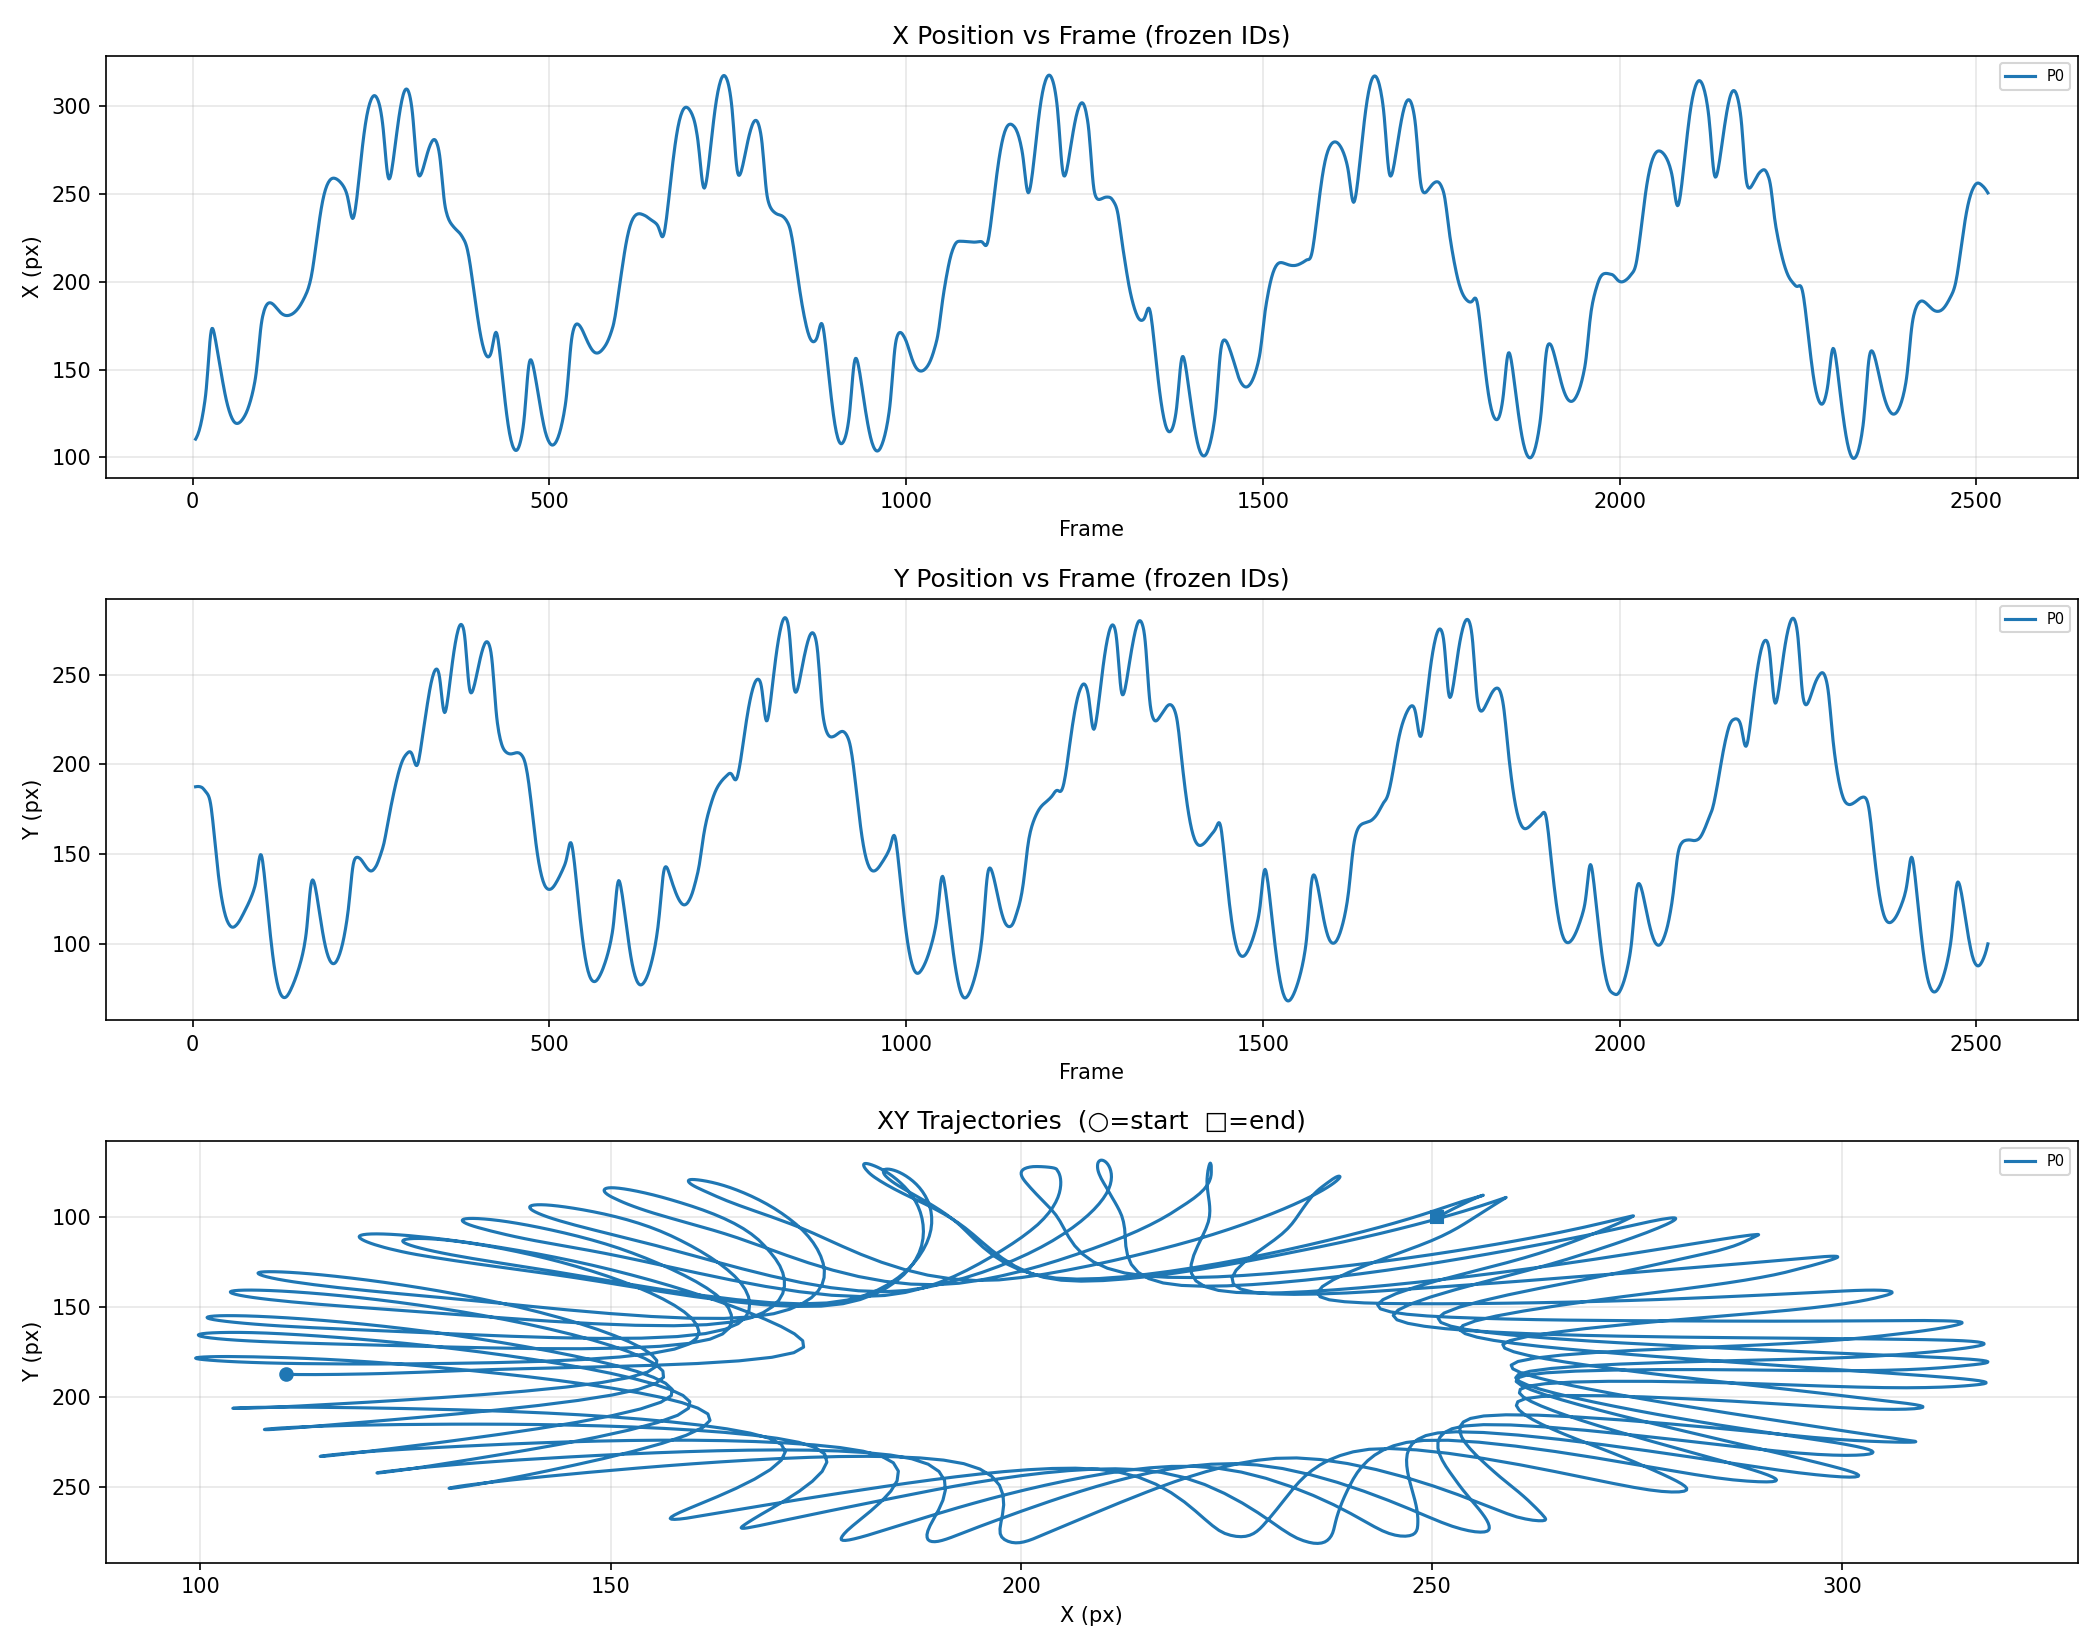
\includegraphics[width=\columnwidth]{one_particle_result.png}
\caption{Single-particle trajectory.}
\label{fig:single_traj}
\end{figure}


\textbf{Two-Particle Trajectory.} The pipeline successfully recovers both particle trajectories across the full duration of the two-particle video without identity switching. The reconstructed $X(t)$ and $Y(t)$ show that both particles have clear periodic behavior with similar amplitudes and the same dominant period, which indicates that both particles follow similar orbital motion under the same experimental conditions. One particle consistently lags behind the other by approximately one quarter of the main cycle, and this phase difference remains stable throughout the recording.

In the $XY$ plane, both particles trace overlapping ring-like orbits around the same hollow central region. The trajectories intersect many times, creating situations where identity tracking becomes difficult because the particles occupy nearby positions. Despite these repeated crossings, the pipeline preserves consistent particle identities across the entire recording. This is achieved by the freeze-identity merging stage, which establishes particle identities early in the sequence using their initial motion patterns and prevents identity exchange during close encounters. 

\begin{figure}[H]
\centering
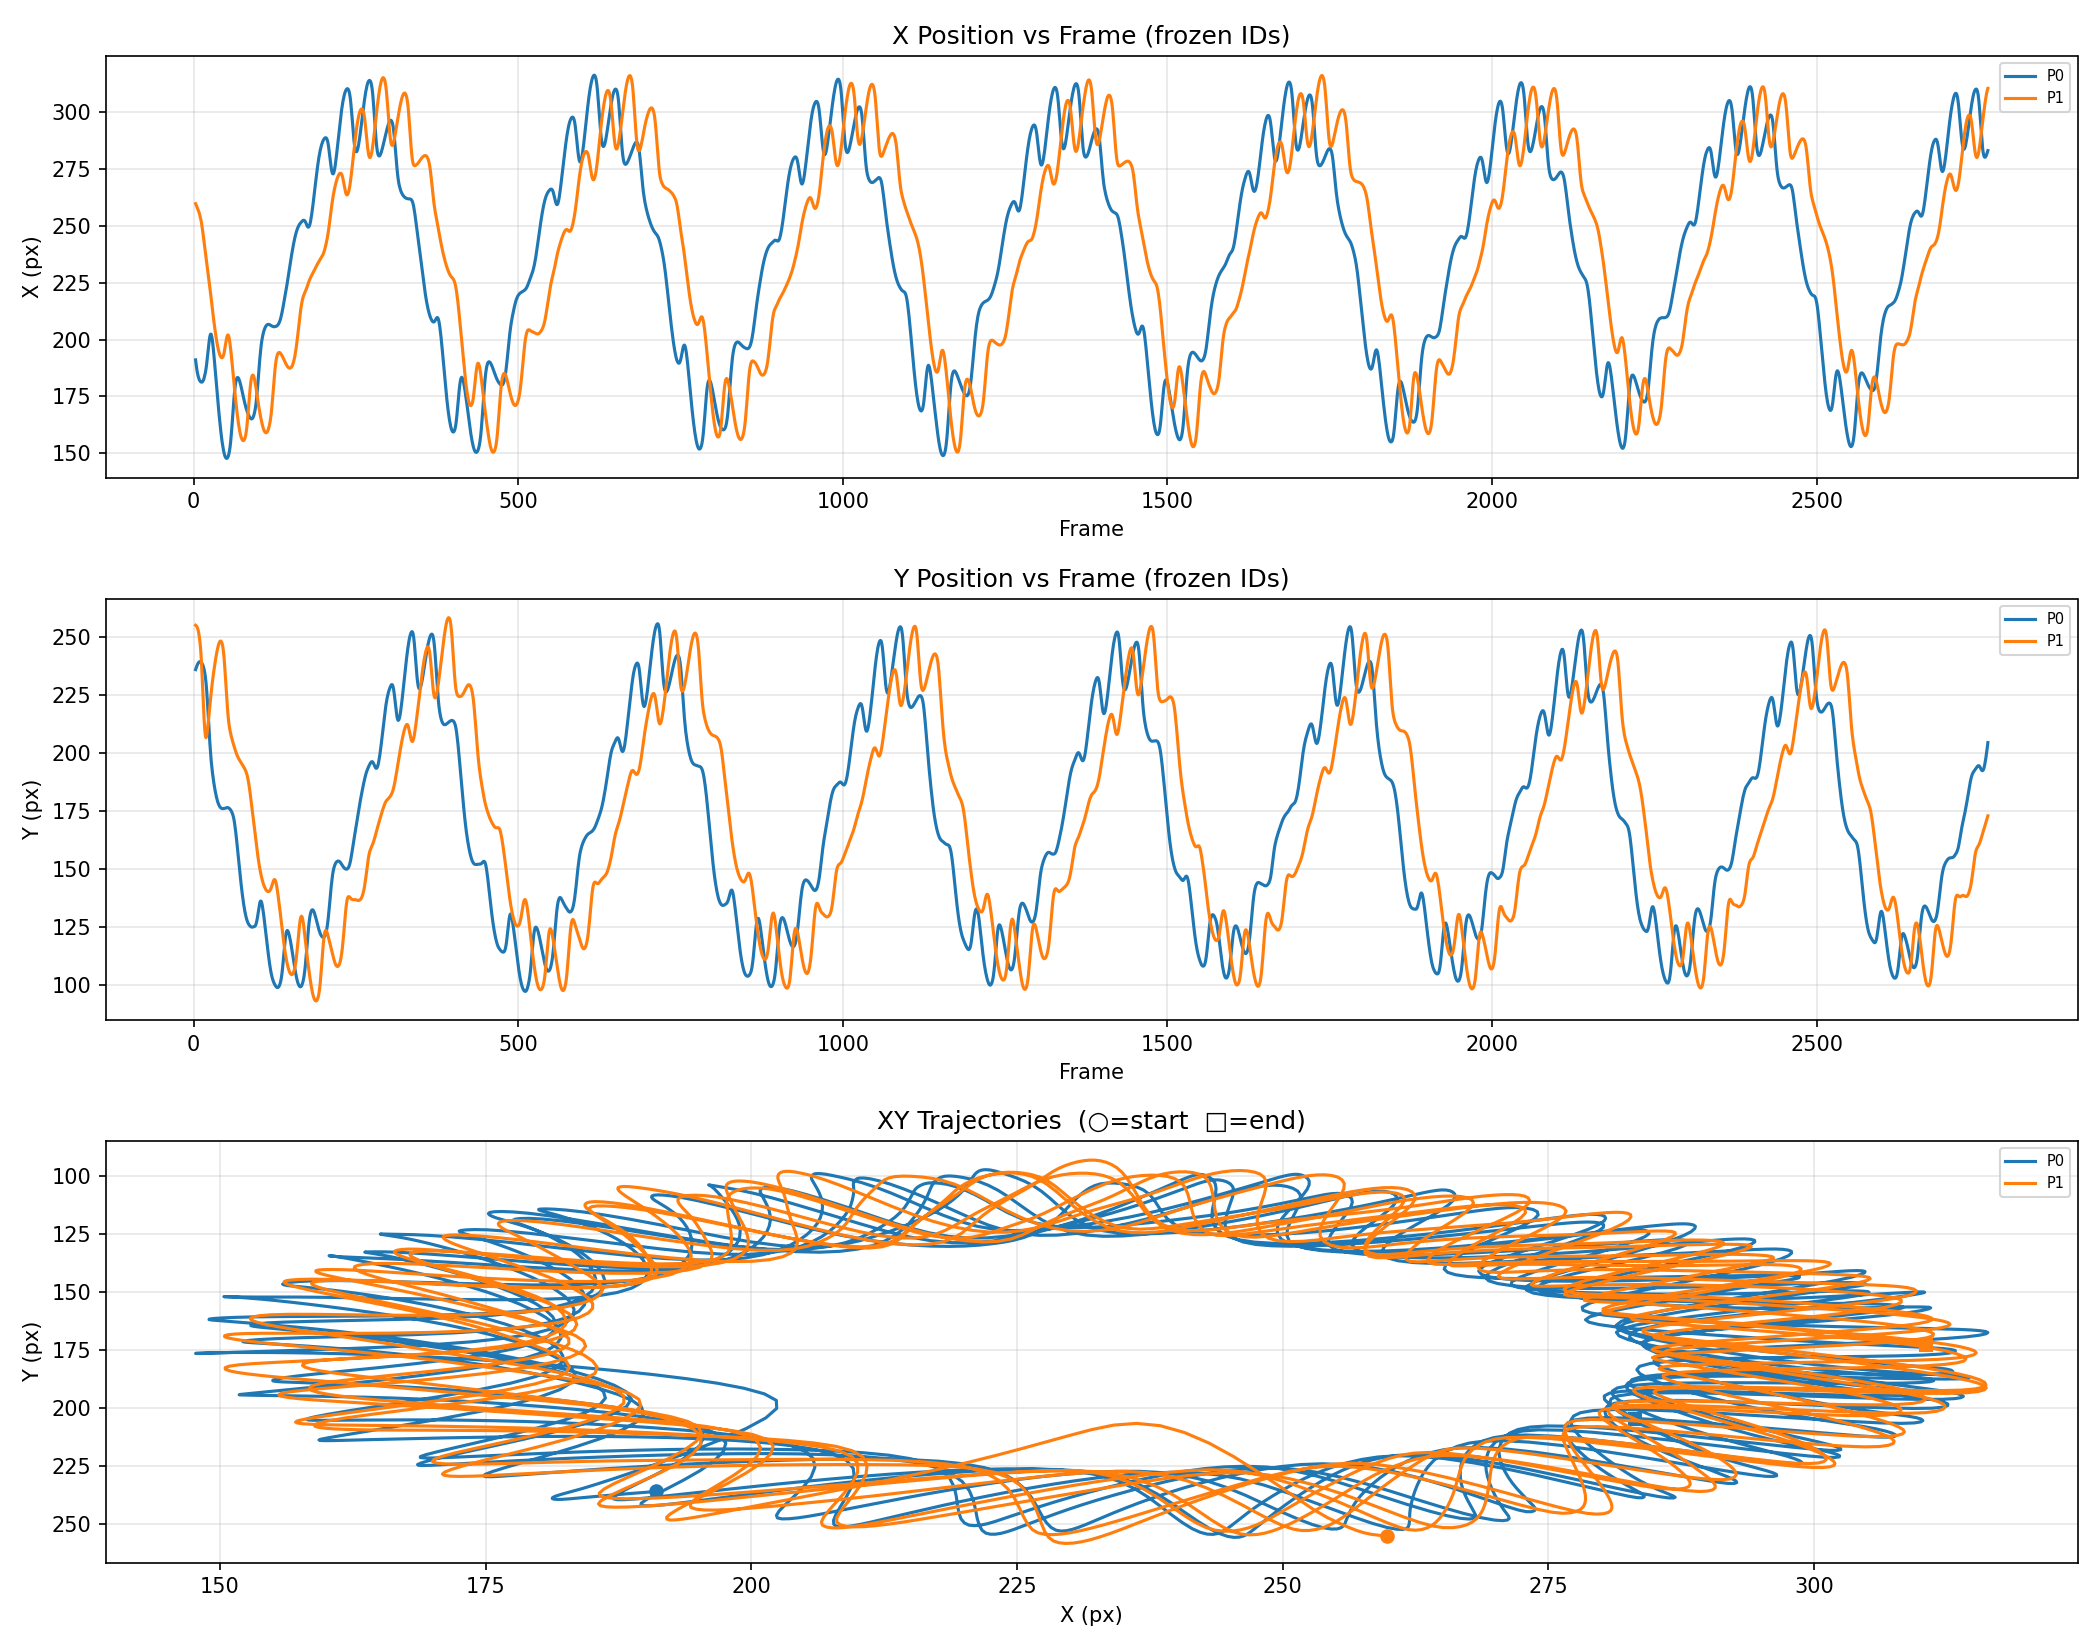
\includegraphics[width=0.90\columnwidth]{two_particle_result.png}
\caption{Two-particle trajectory.}
\label{fig:single_traj}
\end{figure}

\textbf{Three-Particle Trajectory.} The pipeline initializes three particle trajectories (P0, P1, and P2). P0 continues throughout the full recording, while P1 and P2 end around frames 368 and 375 after the particles come very close and their mask regions merge together. This can be seen directly in the $X(t)$ and $Y(t)$ plots, where the P1 and P2 signals stop early, while the P0 signal continues until the end of the video.

After the merge, the combined mask is assigned to the longest-lasting identity (P0). When the particles separate again, the pipeline continues tracking them as part of P0 instead of recovering the original identities of P1 and P2. As a result, the final $XY$ trajectory becomes a tangled combined path instead of the stable ring-like trajectories observed in the one- and two-particle cases.

This represents the current limitation of the pipeline. The main reason is that SAM 2 tracks one connected mask for each identity. When multiple particle masks merge into a single region, the pipeline cannot later separate them back into their original identities after they split apart again. This limitation is discussed further in Section~\ref{sec:limitations}.

\begin{figure}[H]
\centering
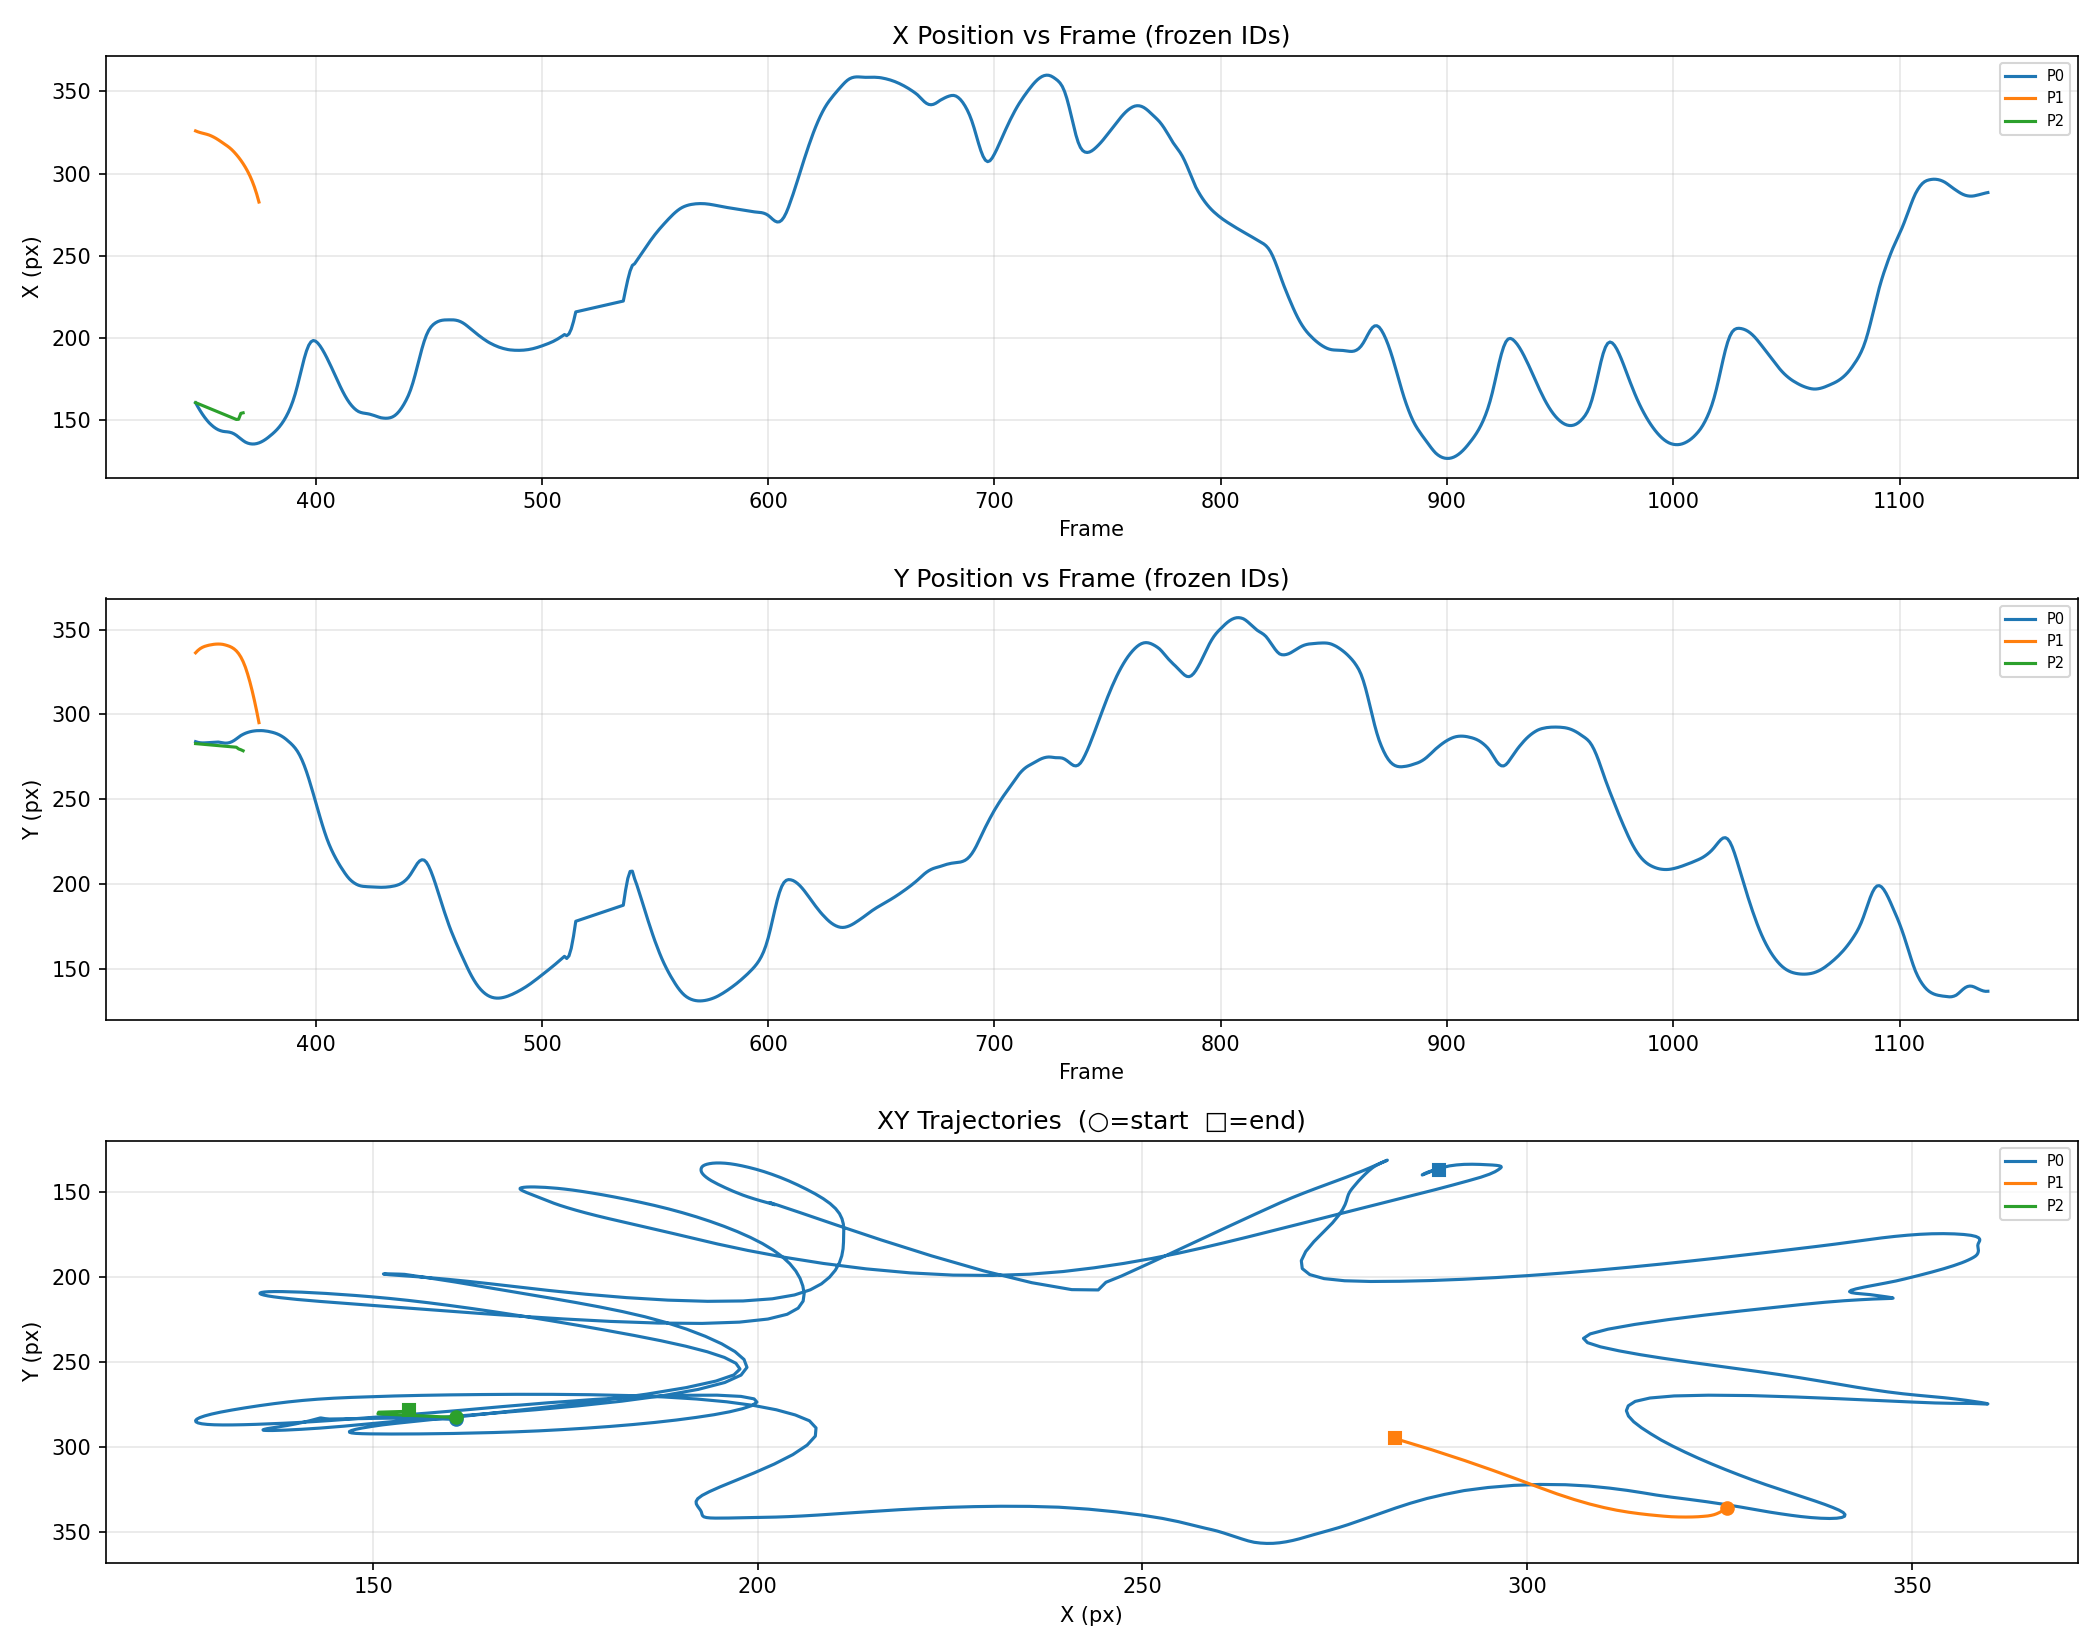
\includegraphics[width=0.95\columnwidth]{three_particle_result.png}
\caption{Three-particle trajectory.}
\label{fig:single_traj}
\end{figure}

\subsection{Evaluation Metrics}
\label{sec:manual-annotation-overlay}

\textbf{Manual-Annotation Overlay.} Validation is performed by independently re-annotating a sparse set of frames from each video and comparing the resulting manual centroids to the pipeline's reconstructed positions. In the single-particle case, 25 frames were annotated, producing 25 matched pairs. In the two-particle case, 13 frames were annotated, yielding 26 matched pairs. In the three-particle case, 8 matched pairs for P0 and P1 within the valid window were provided.

Figure~\ref{fig:overlay_pic} shows the displacement-from-start trajectories for each video, with the pipeline output drawn as a continuous curve and manual annotations plotted as discrete points. The manual points lie close to the pipeline curve in all three videos, with the smallest deviations between manual and pipeline centroids in the single- and two-particle cases. 

Quantitative errors are summarized in Table~\ref{tab:overlay}: the single- and two-particle cases yield mean errors of approximately 15 px, on the order of one particle diameter, while the three-particle case shows substantially larger errors which restates the results obtained above. 

\begin{figure}[H]
\centering
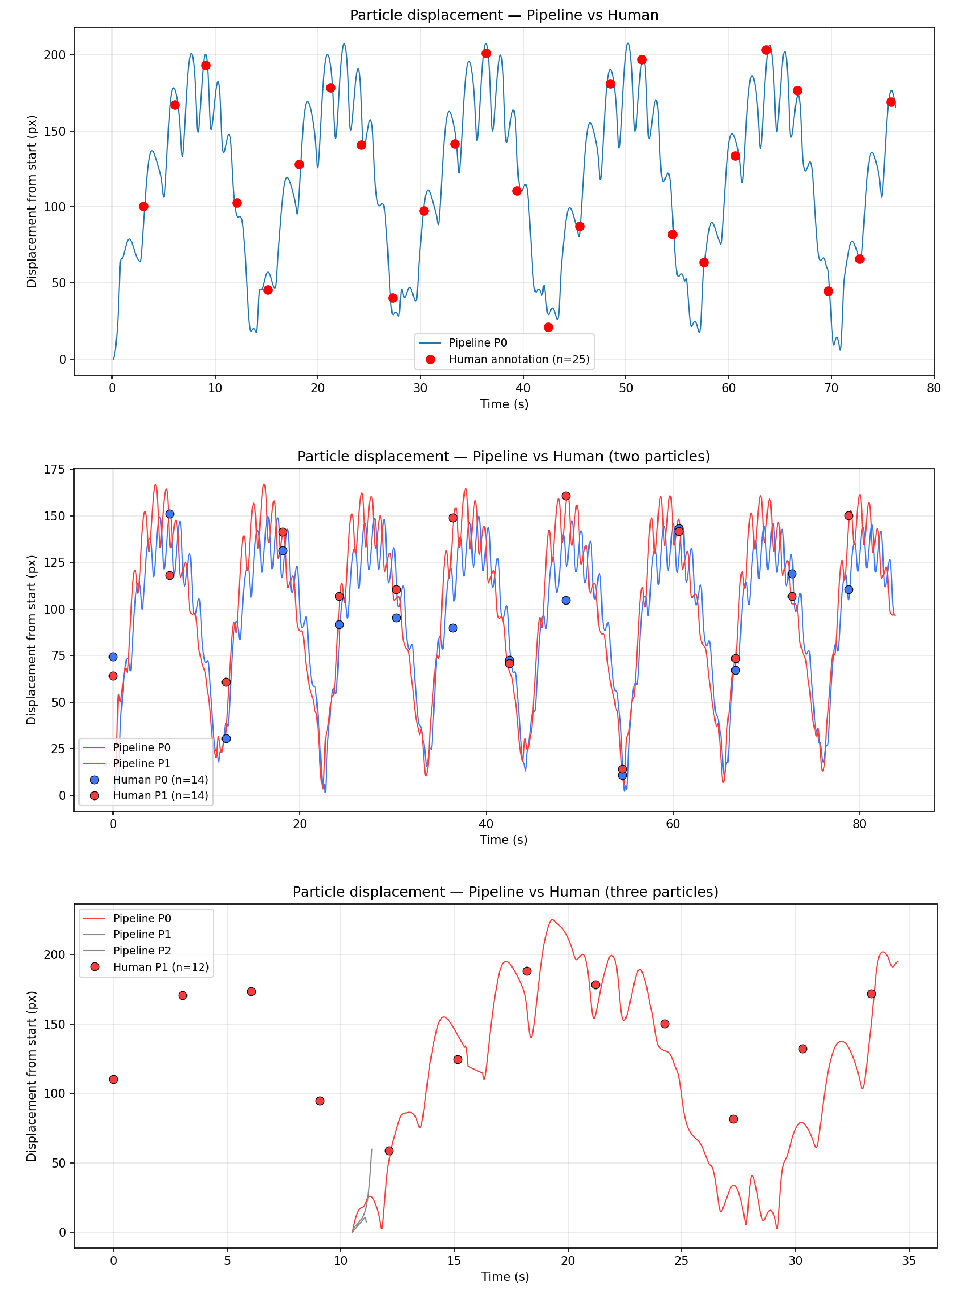
\includegraphics[width=1.03\columnwidth]{overlay cases final.pdf}
\caption{Manual-Annotation Overlay}
\label{fig:overlay_pic}
\end{figure}


\begin{table}[H]
\caption{Manual-annotation overlay error per video}
\label{tab:overlay}
\centering
\begin{tabular}{lccccc}
\toprule
Video & $n$ & Mean & Median & Std & 95th pct \\
\midrule
One-particle    & 25 & 15.49 & 14.73 & 7.05 & 27.69 \\
Two-particle    & 26 & 15.00 & 13.69 & 8.45 & 31.22 \\
\quad P0 only       & 13 & 16.13 & 13.89 & -- & -- \\
\quad P1 only       & 13 & 13.87 & 13.15 & -- & -- \\
Three-particle  & 8 & 43.74 & 28.30 & 30.98 & 99.21 \\
\bottomrule
\end{tabular}
\end{table}


\section{Discussion}

\subsection{Identity Preservation}

The two-particle case provides the most informative test for the proposed pipeline. The classical CV baseline produced severe identity fragmentation in the single-particle setting, generating many distinct identifiers for a single physical particle. The YOLO-only configuration improved per-frame localization greatly, but, again, wasn't able to mitigate the issue of identity switches, since per-frame detection provides no inter-frame correspondence. In contrast, the proposed method preserved both particle identities across the full recording of more than 2,500 frames, including during repeated XY-plane crossings.

The similar localization errors in the single- and two-particle cases (mean 15.49 px vs. 15.00 px) further indicate that introducing a second particle did not noticeably reduce tracking accuracy, and the per-particle errors within the two-particle case are nearly symmetric (16.13 px for P0, 13.87 px for P1). These results confirm that the freeze-identity merging stage maintains stable particle identities over time: starting motion signatures distinguish particles whose orbits later cross, and the per-frame consistency filter rejects positions that would correspond to identity exchange during a crossing. 

\subsection{Error magnitude}

The mean localization error in the valid operating regime was approximately 15 px, which is about the size of one particle diameter at the used imaging scale. This error mainly comes from the limitations of manual annotation rather than from tracking failure. The manual particle positions were estimated using hand-drawn bounding boxes, while the pipeline calculated centroids directly from SAM 2 segmentation masks. Although both methods refer to the same particle, they can place the center slightly differently near the particle boundaries.

The error values in the single-particle and two-particle cases were very similar (15.49 px and 15.00 px), suggesting that the remaining error is mostly caused by the annotation process and not by the tracking itself. A more accurate evaluation would require pixel-level segmentation annotations instead of bounding boxes, which is left for future work.

\subsection{Three-particle Case: Current Limitation}
\label{sec:limitations}

The three-particle case defines the current limit of the pipeline. During close encounters, the masks of multiple particles merged into a single connected region in the SAM 2 output. After merging, the tracker assigned the combined mask to the dominant identity (P0), causing P1 and P2 to be lost permanently around frames 368 and 375. From that point onward, P0 absorbed the motion of all three particles, and the reconstructed trajectory no longer represented the true motion of the individual particles.

The increased localization error in this case quantitatively reflects this case's limitation: a mean error of 43.74 px and 95th percentile of 99.21 px in the three-particle video, compared to approximately 15 px and 30 px, respectively, for the single- and two-particle cases. The pipeline is therefore not reliable for dense multi-particle interactions in its current form. SAM 2 maintains one connected mask per identity, so when two particles produce a single connected mask, there is no mechanism in the pipeline to split the merged component back into separate identities once the particles physically separate. Resolving this failure would require an additional re-identification stage that detects when a merged mask splits into multiple components and re-binds identities to the resulting fragments.


\section{Conclusion}

This work developed and evaluated a data-driven pipeline for particle detection and trajectory reconstruction in free-surface liquid crystal microscopy videos. The proposed method combines a fine-tuned YOLO detector for per-frame localization, the SAM 2 video predictor for mask-based identity propagation, and a signature-based freeze-identity merging stage that resolves residual fragmentation by fixing each particle's identity early in the recording and admitting later positions only when consistent with the established trajectory. The pipeline successfully reconstructed stable periodic trajectories in the single-particle case across more than 2,500 frames, preserved both particle identities through repeated trajectory crossings in the two-particle case, and identified a clear limitation during dense multi-particle interactions where the masks of distinct particles merge into a single connected component because of frequent collisions. Manual validation confirmed agreement between reconstructed and annotated trajectories within approximately one particle diameter in the first two cases. The results demonstrate that combining modern detection and segmentation models with trajectory-aware identity recovery is an effective strategy for particle tracking in anisotropic soft-matter microscopy, where classical particle trackers and general-purpose multi-object trackers do not transfer cleanly. The freeze-identity merging stage, in particular, could be applied to other microscopy domains where particles or cells change appearance and need to be tracked through close encounters.

\section{Future Work}

The most direct next step is resolving collision-caused identity merging by introducing a re-identification stage capable of recovering particles after merged masks split into separate regions again. Additional improvements include pixel-level manual annotation for more precise validation and evaluation on denser particle systems with more frequent close interactions. Future work will also focus on extending the pipeline to denser multi-particle configurations, where similar collision-induced complex interactions are expected to occur more frequently, and robust re-identification in this case becomes essential.

\section*{Acknowledgements}

I would like to express my sincere gratitude to my supervisor, Aleksandr Hayrapetyan, for his valuable guidance and support throughout this research project. I also thank Dr. Sergey Shvetsov and the Institute of Physics at Yerevan State University for providing the experimental video data on which this work is based.

\bibliographystyle{IEEEtran}
\bibliography{references}

\end{document}